\documentclass[11pt]{article}
\usepackage[T1]{fontenc}
\usepackage{pdfpages}
\usepackage[hidelinks]{hyperref}

\begin{document}

\begingroup
\sffamily
\hypersetup{linkcolor=black}
\tableofcontents
\endgroup
\clearpage

\phantomsection
\addcontentsline{toc}{section}{Lecture 1 -- Overview}
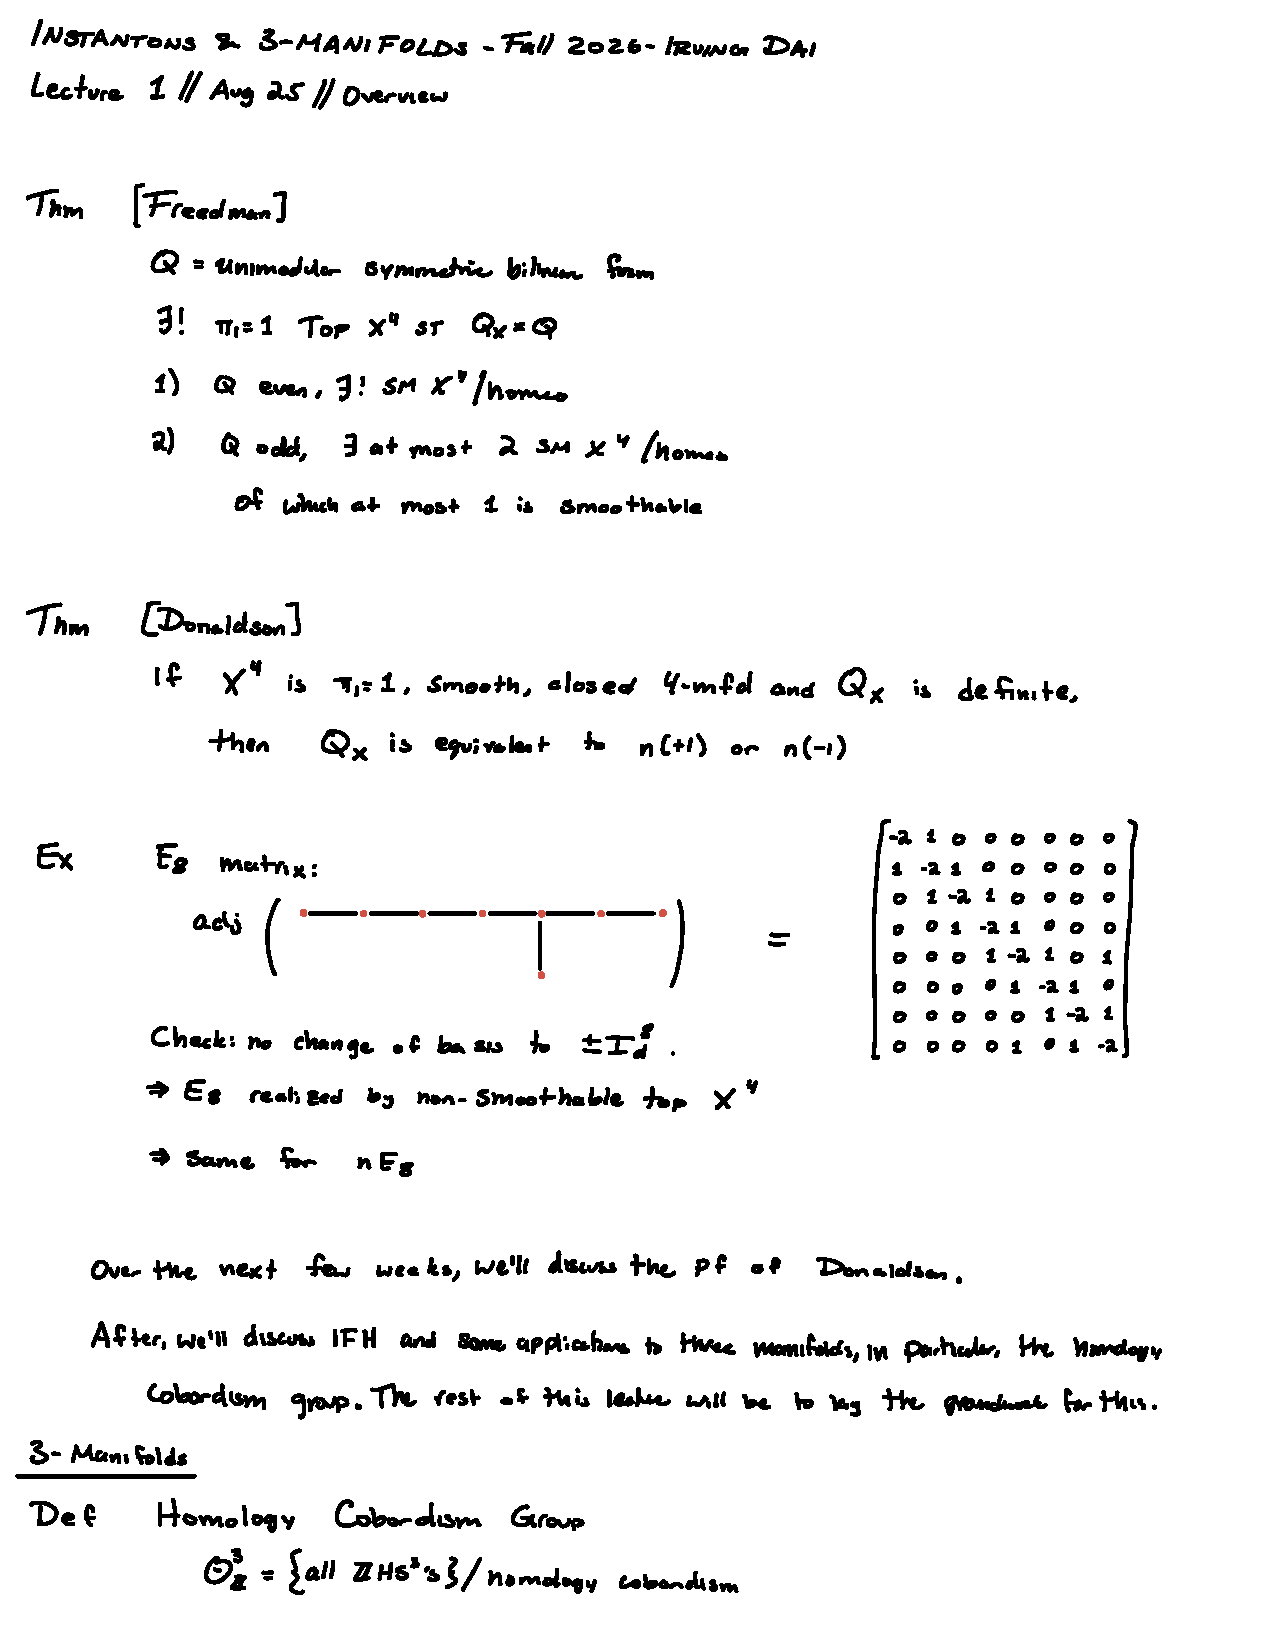
\includepdf[pages=-]{lecture1.pdf}

\phantomsection
\addcontentsline{toc}{section}{Lecture 3 -- Examples \& Hodge Theory}
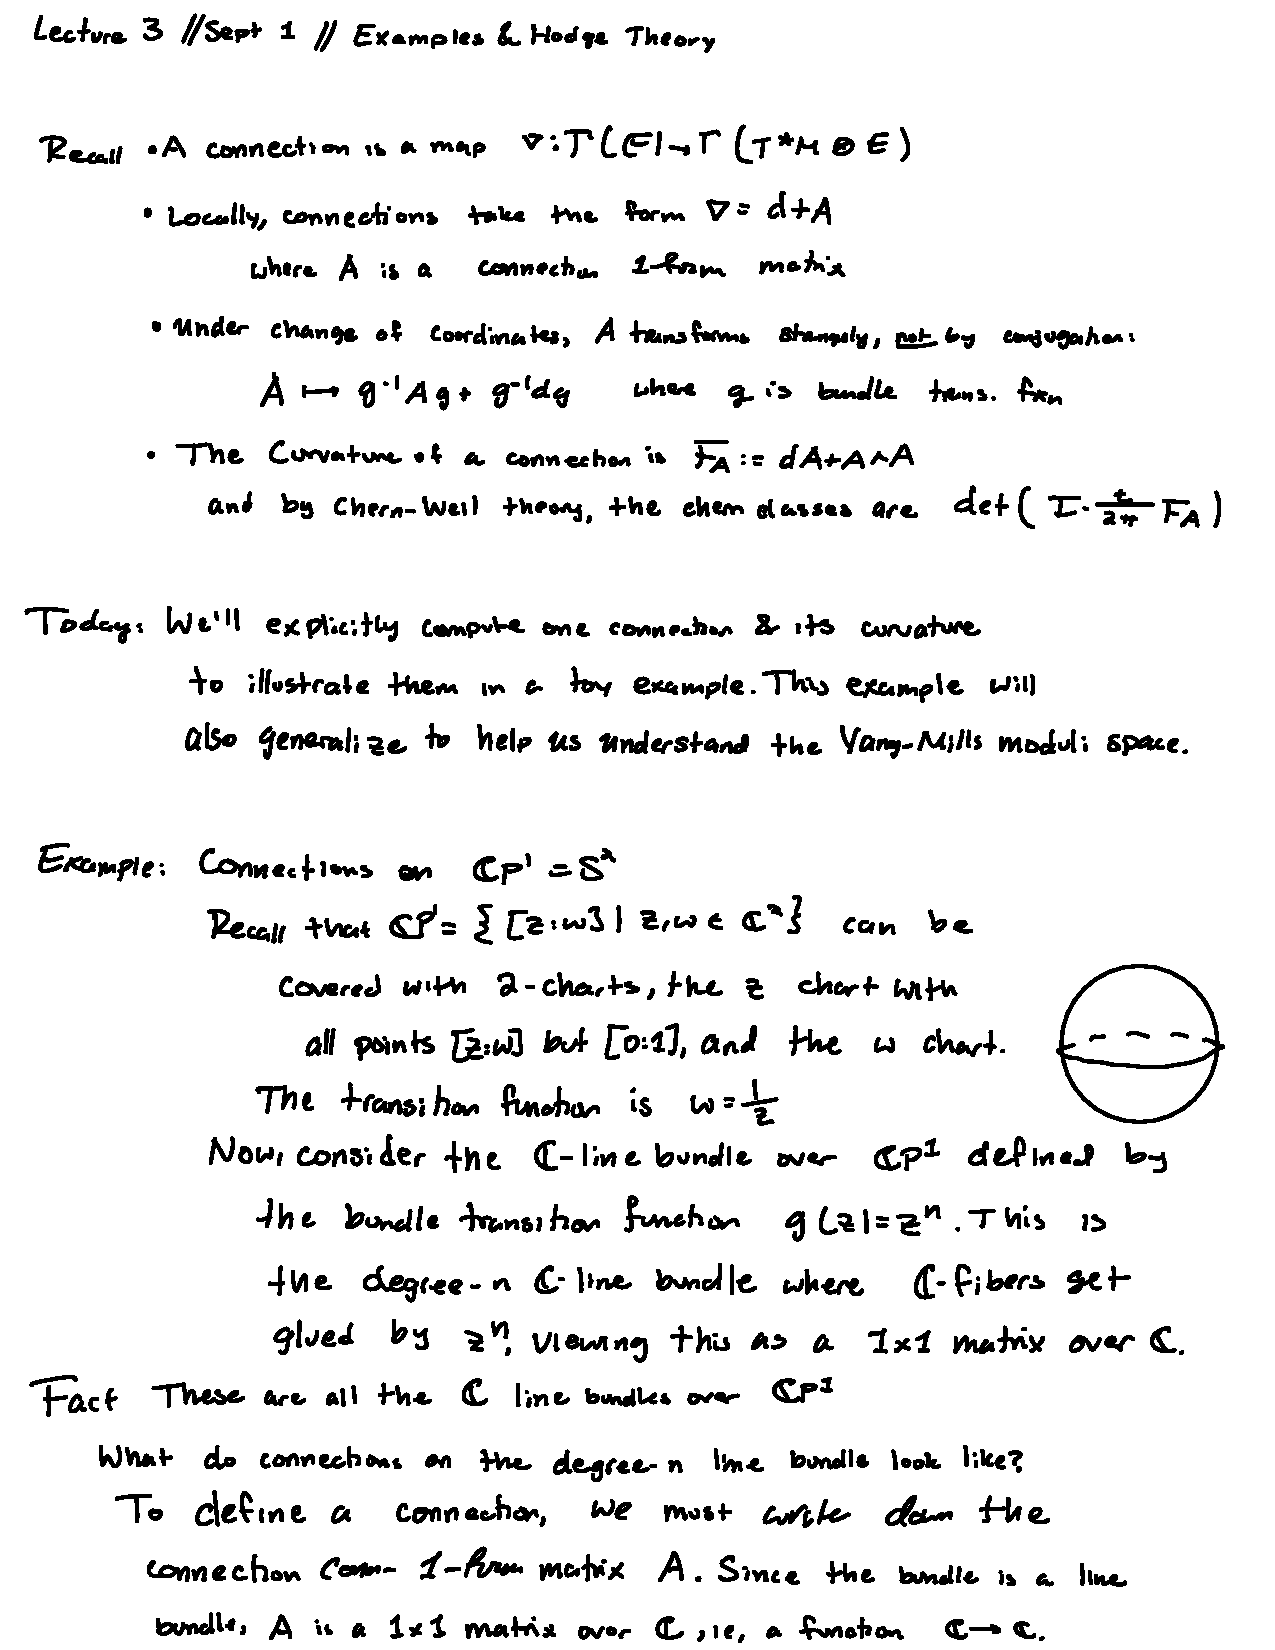
\includepdf[pages=-]{lecture3.pdf}

\phantomsection
\addcontentsline{toc}{section}{Lecture 5 -- Yang Mills Functional \& Equations}
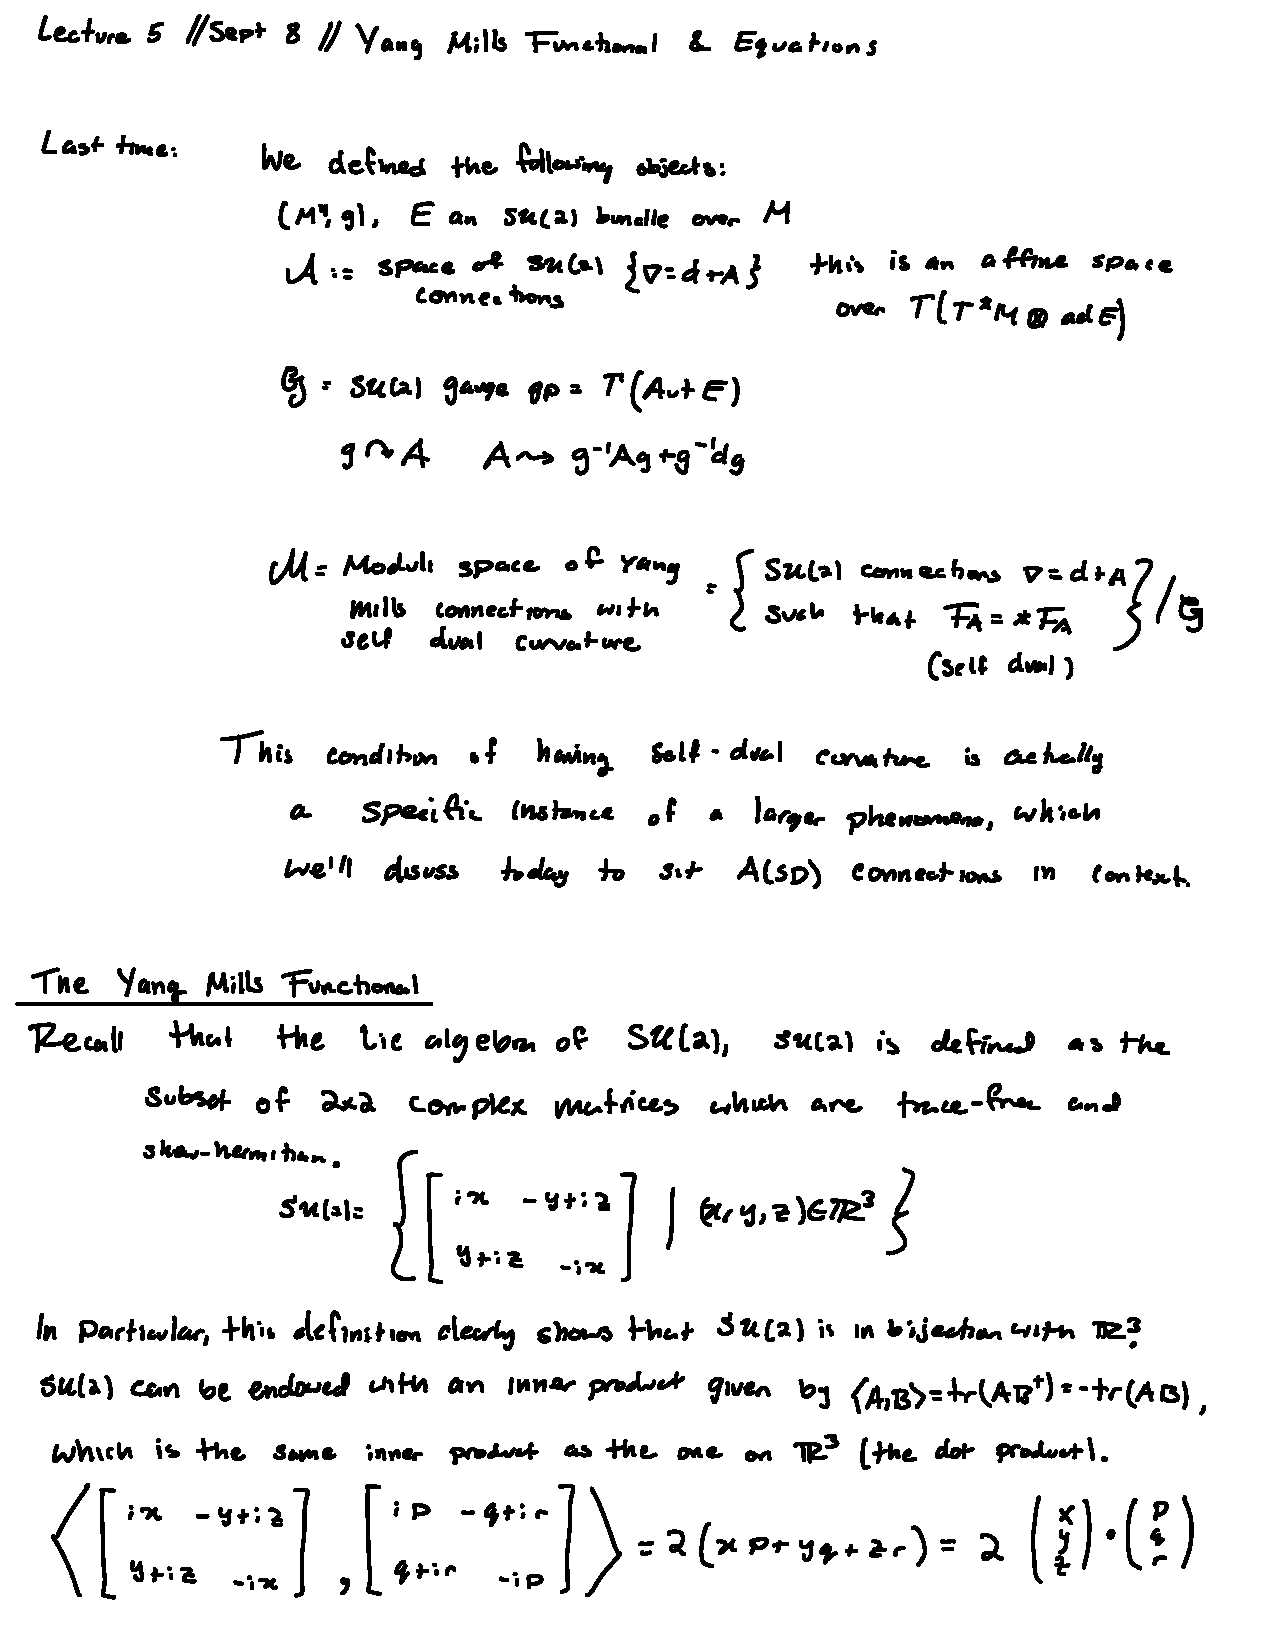
\includepdf[pages=-]{lecture5.pdf}

\phantomsection
\addcontentsline{toc}{section}{Lecture 7 -- Outline of proof of Donaldson's theorem}
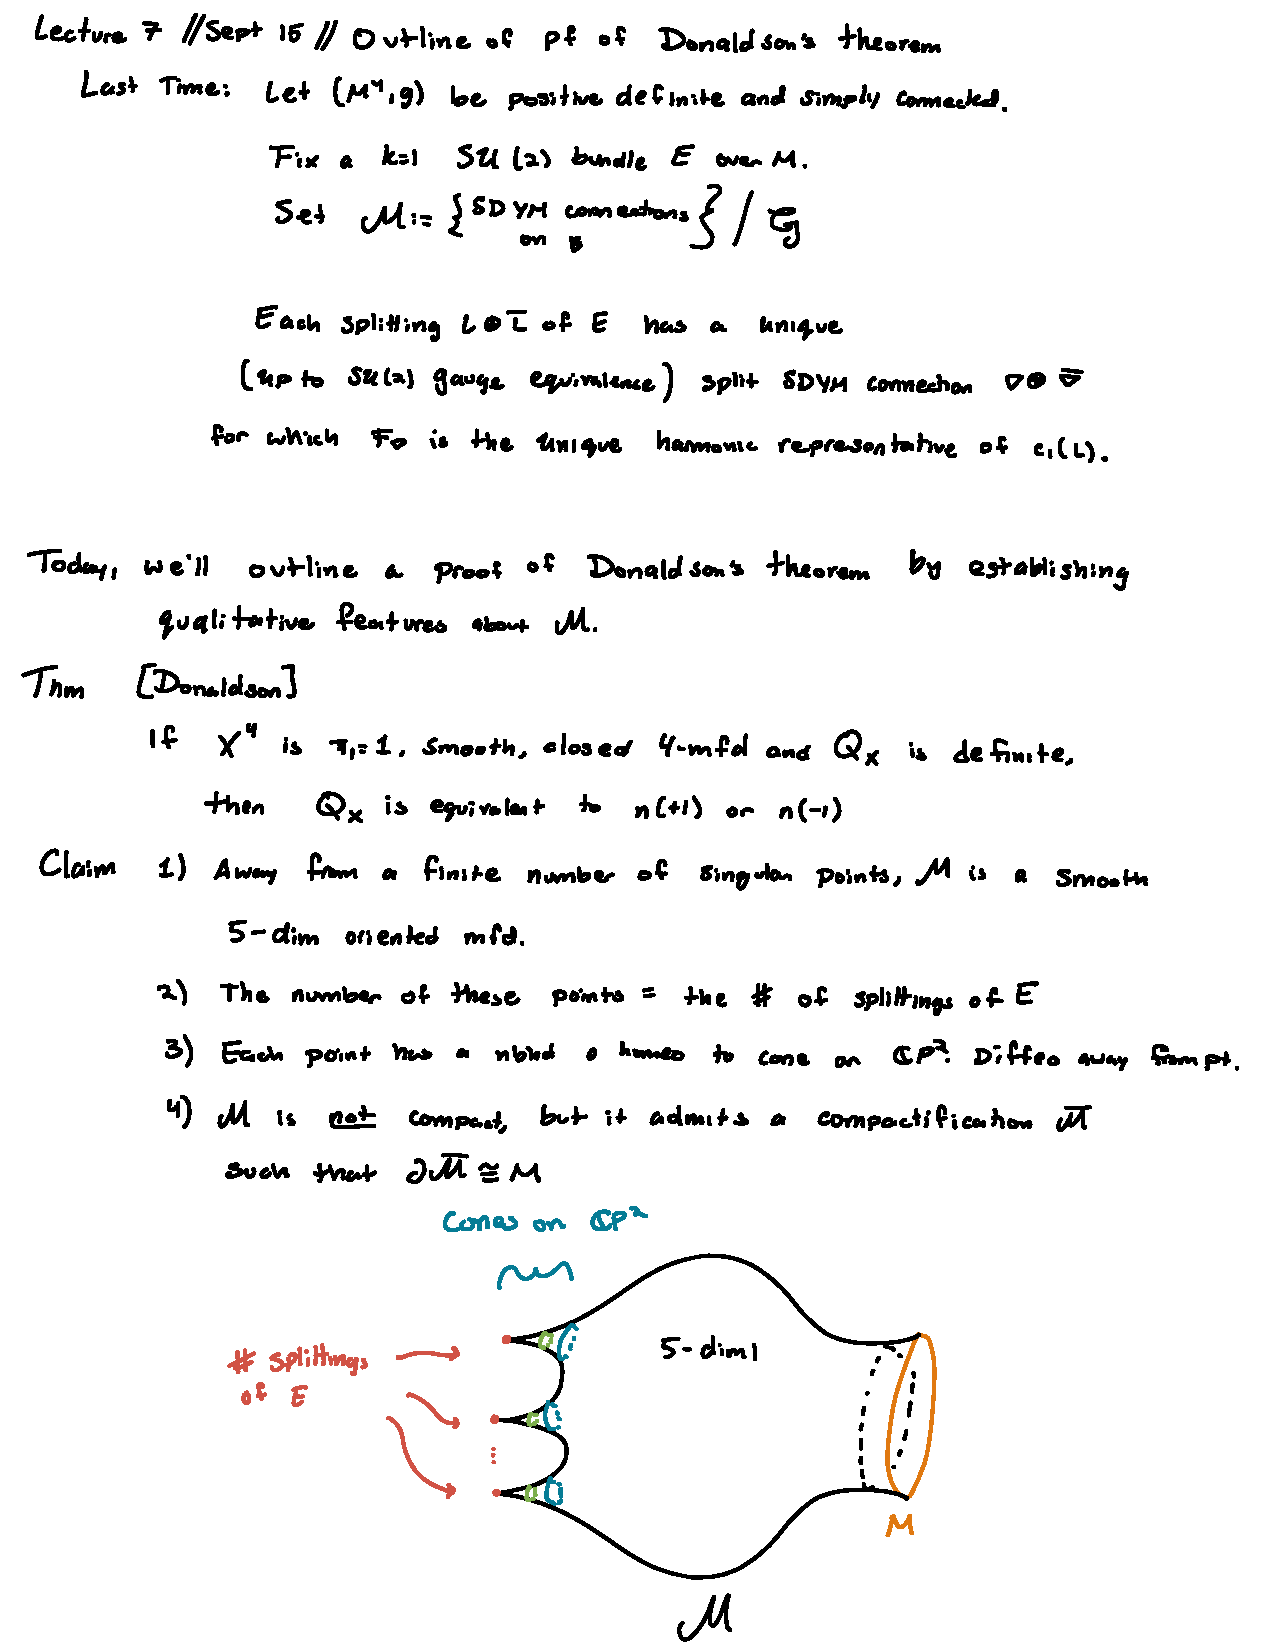
\includepdf[pages=-]{lecture7.pdf}

\phantomsection
\addcontentsline{toc}{section}{Lecture 8 -- Singularities in M and Holonomy}
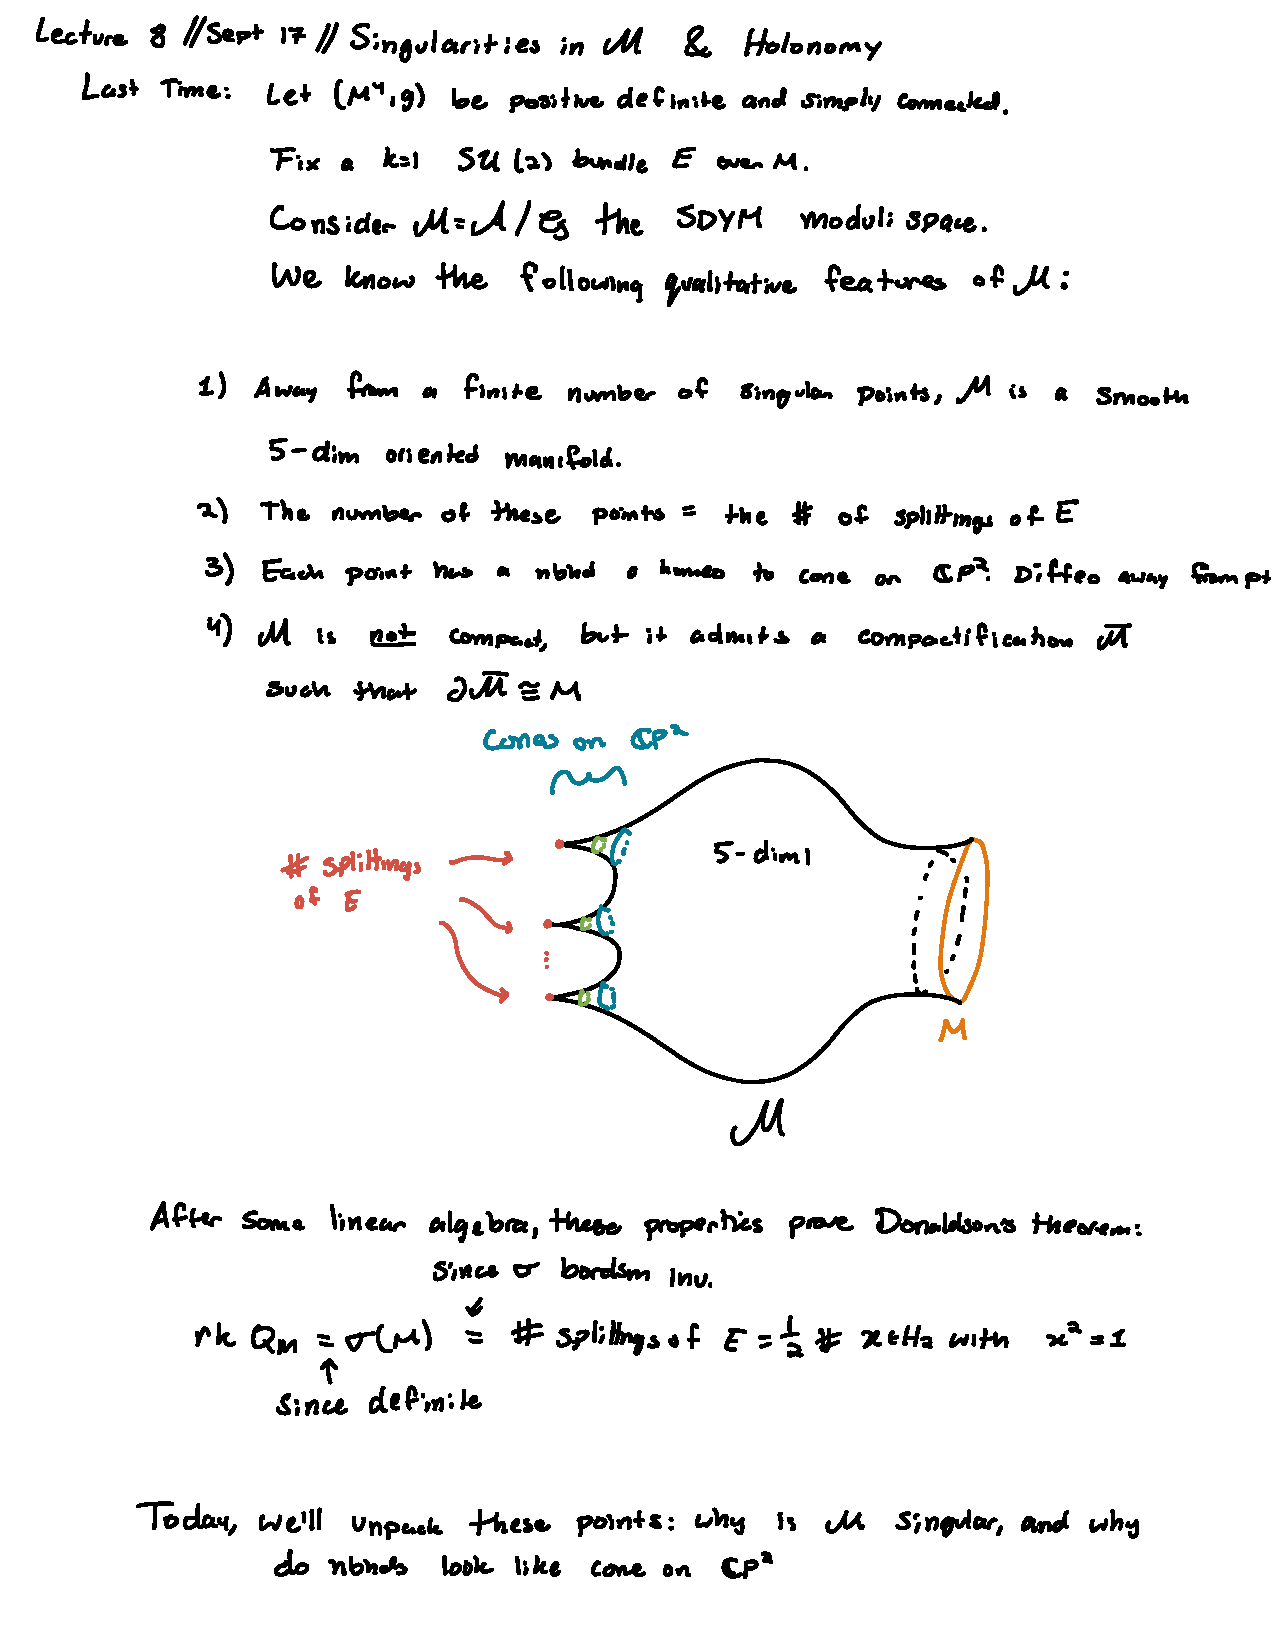
\includepdf[pages=-]{lecture8.pdf}

\phantomsection
\addcontentsline{toc}{section}{Lecture 9 -- Singularities in M, part 2}
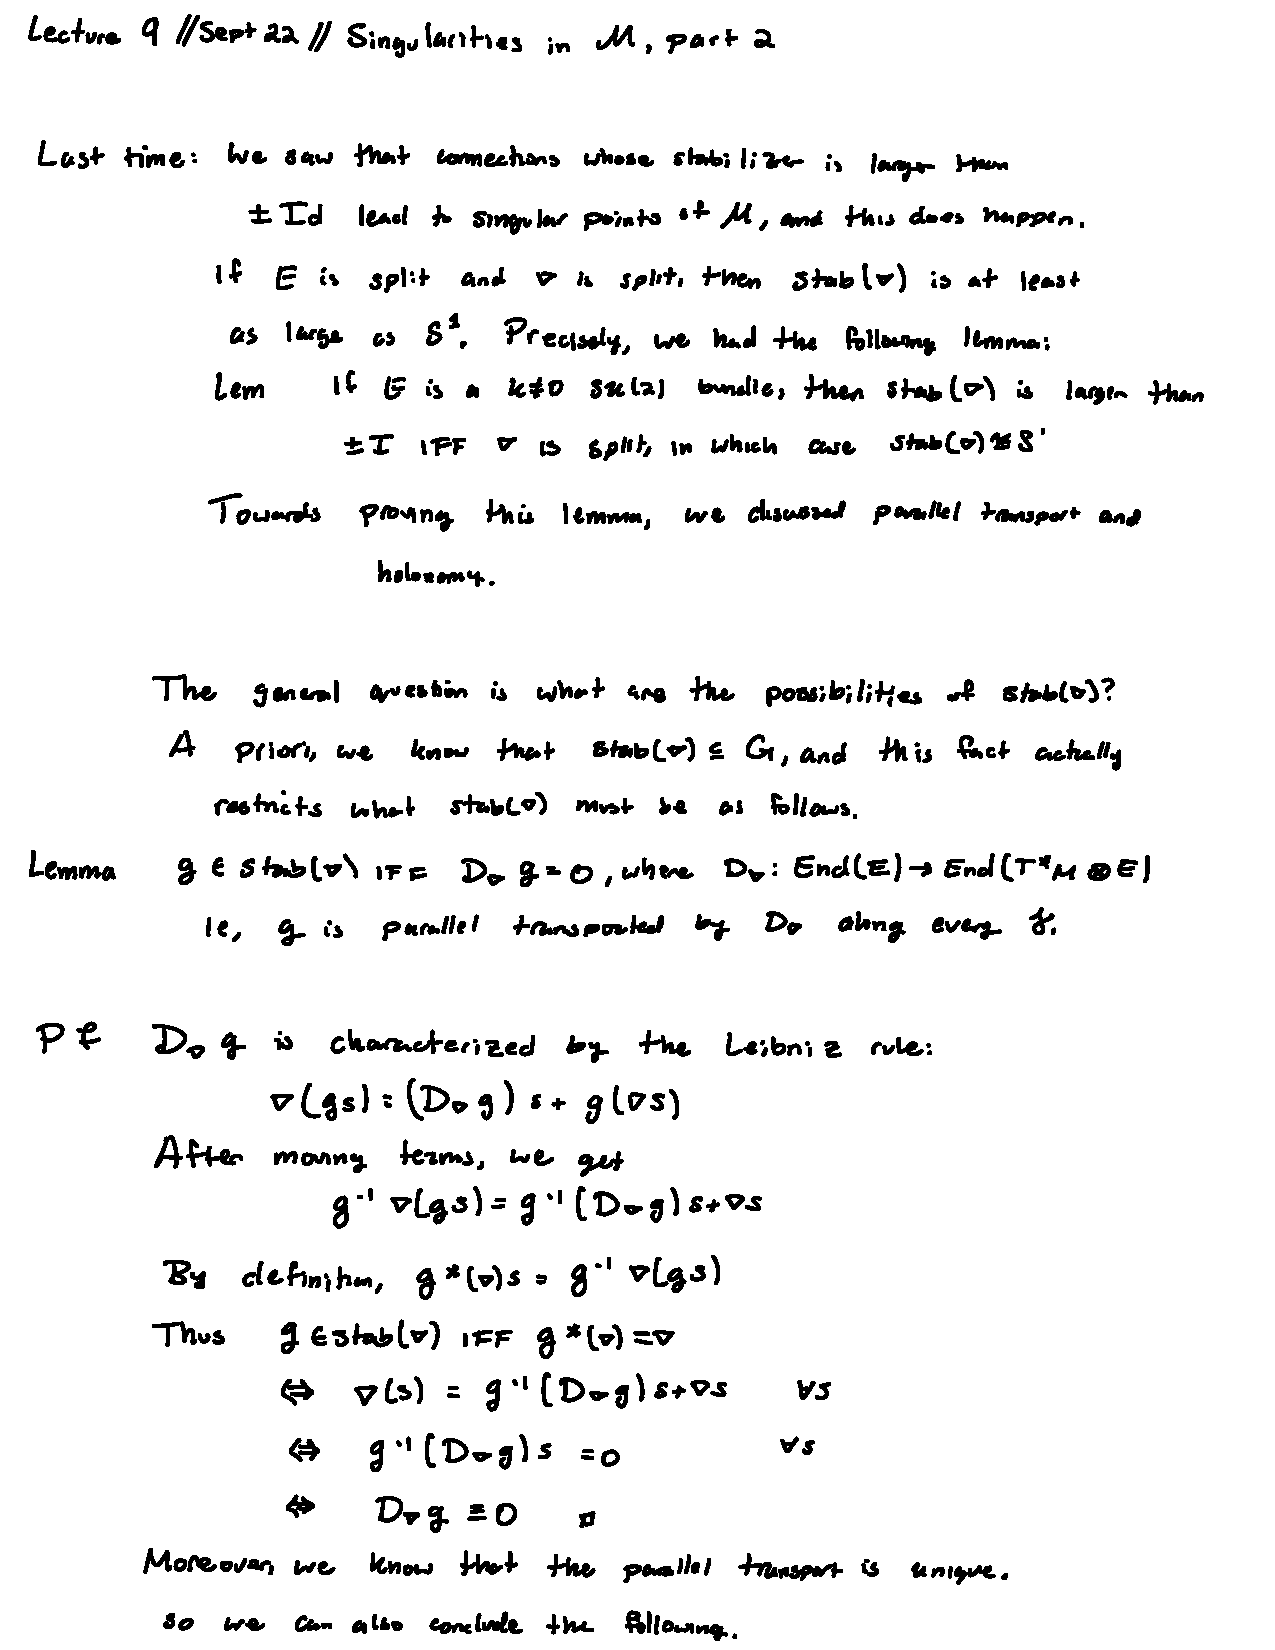
\includepdf[pages=-]{lecture9.pdf}

\phantomsection
\addcontentsline{toc}{section}{Lecture 11 -- Instanton Floer Homology}
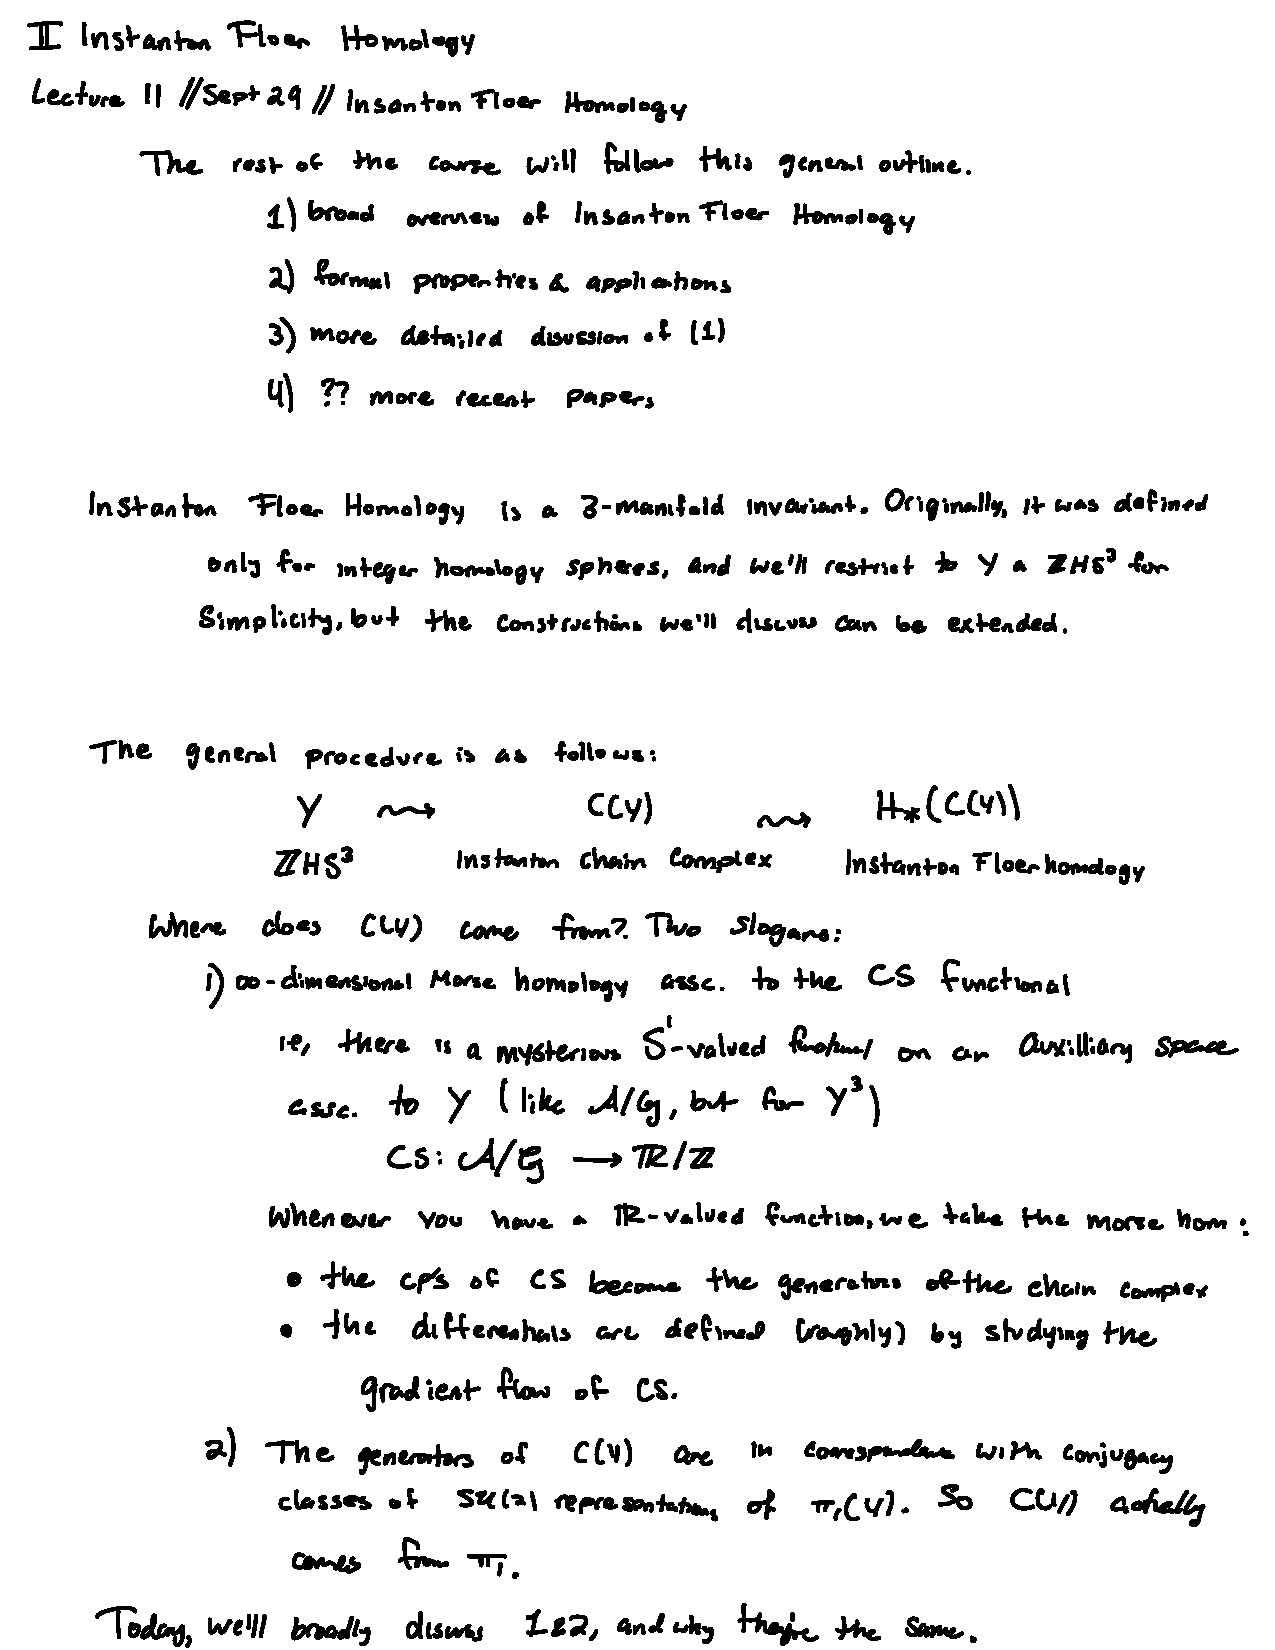
\includepdf[pages=-]{lecture11.pdf}

\phantomsection
\addcontentsline{toc}{section}{Lecture 12 -- The Chern-Simons Functional \& Reducibles}
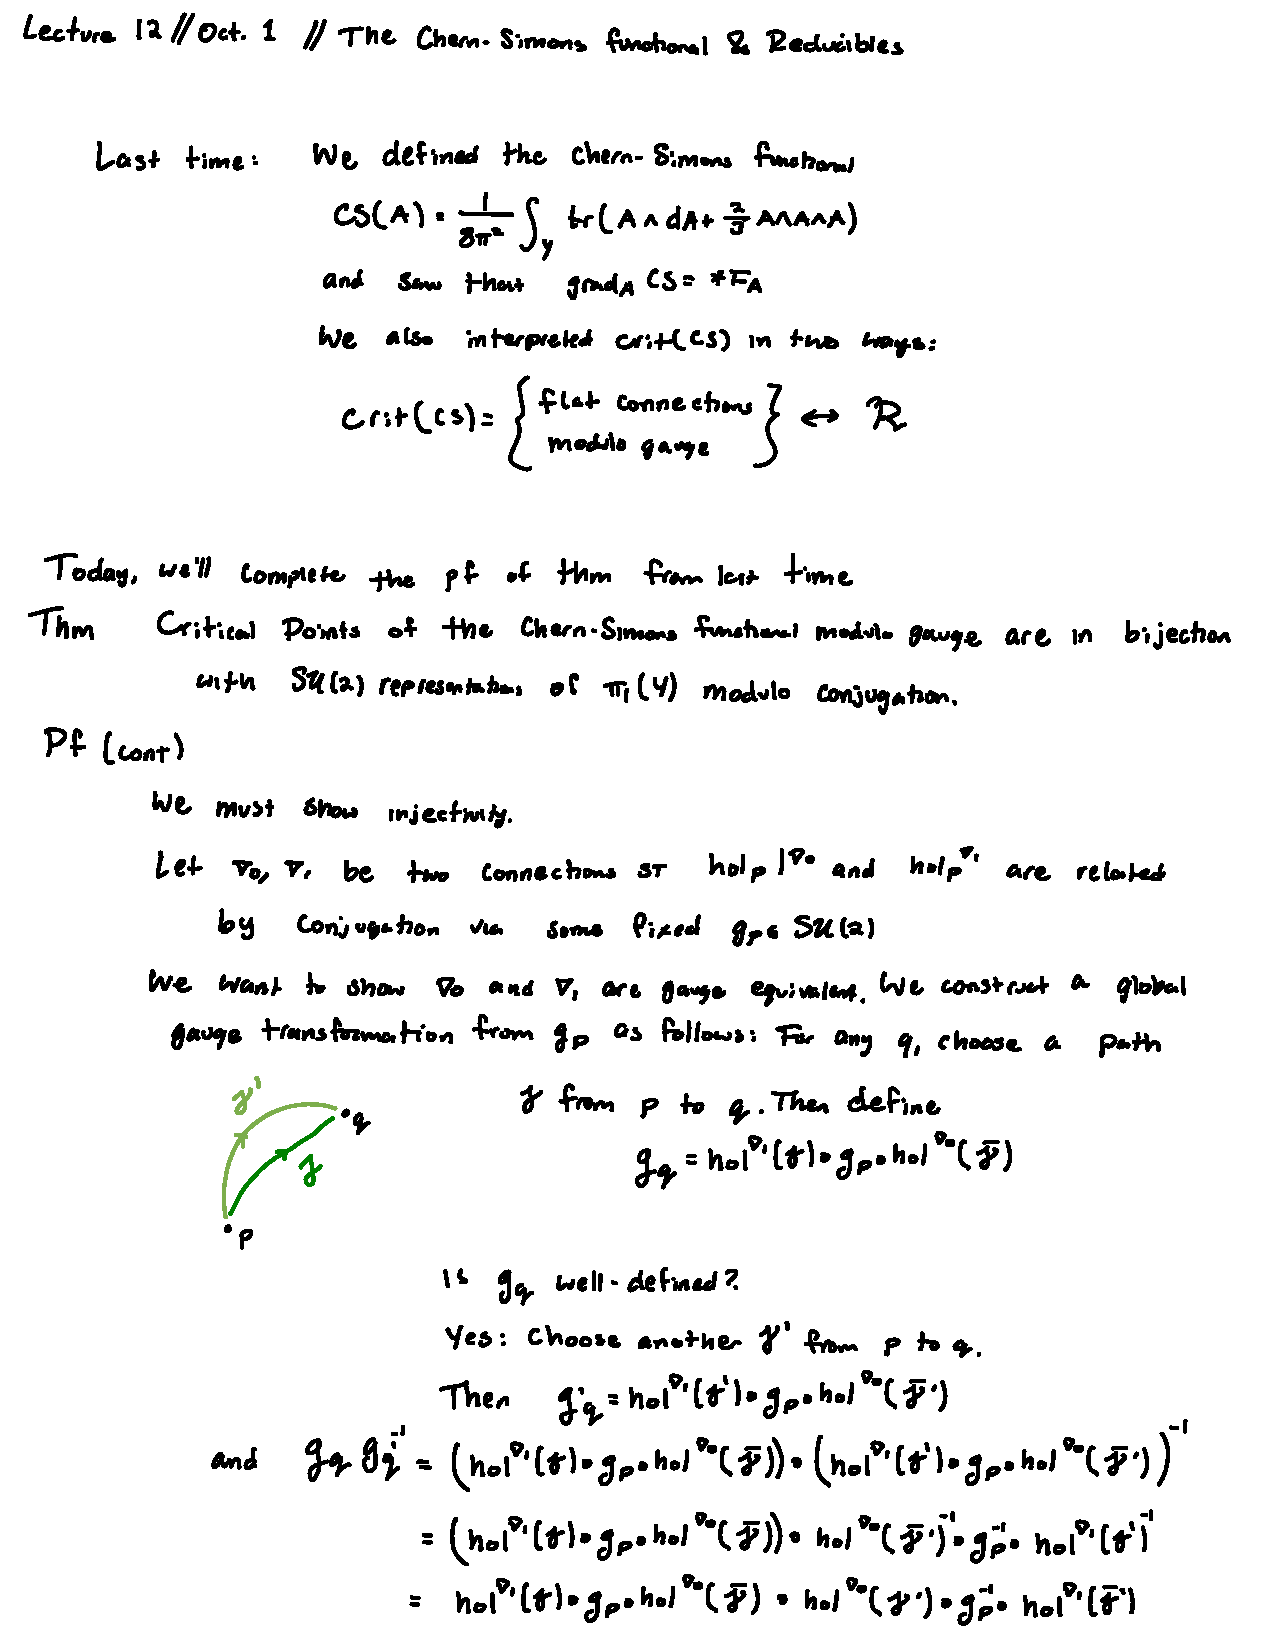
\includepdf[pages=-]{lecture12.pdf}

\phantomsection
\addcontentsline{toc}{section}{Lecture 13 -- Defining Instanton Floer Homology}
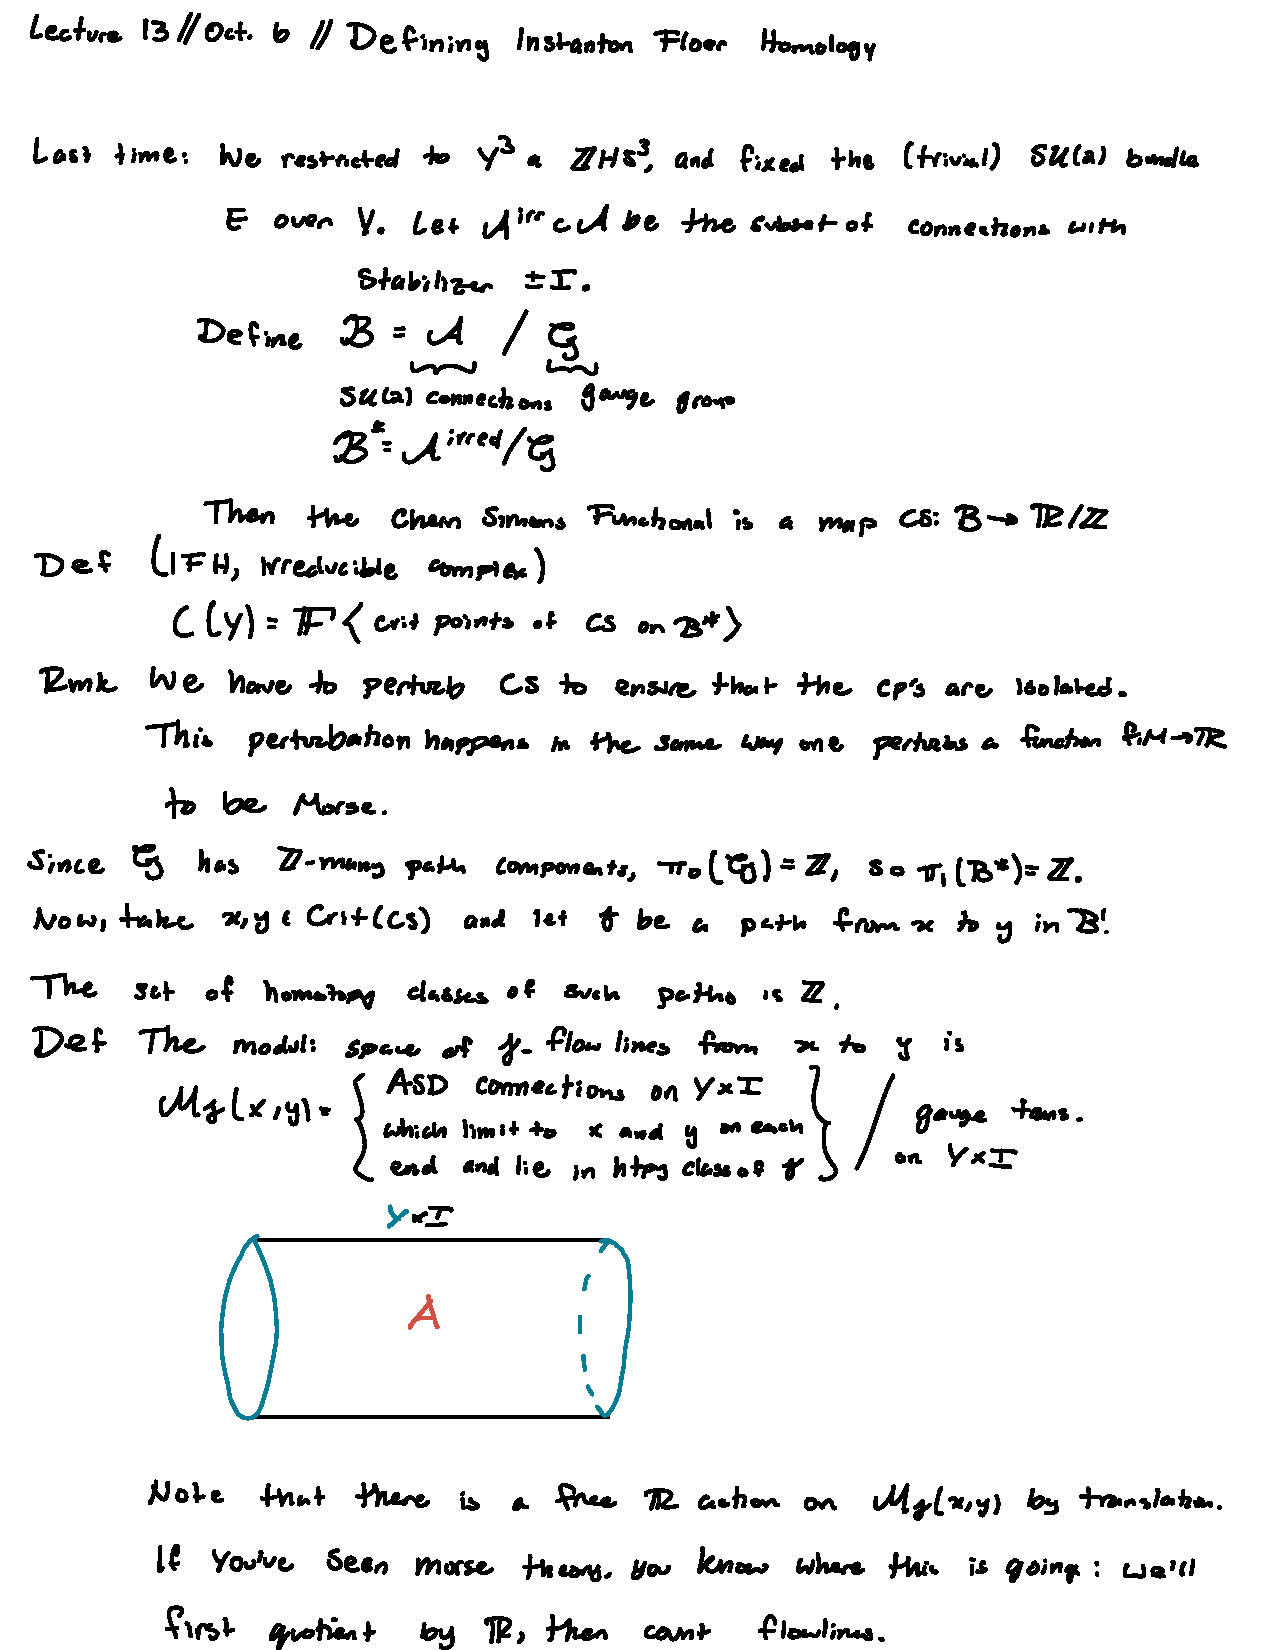
\includepdf[pages=-]{lecture13.pdf}

\phantomsection
\addcontentsline{toc}{section}{Lecture 14 -- Lifting to Z-grading and the Filtered Chain Complex}
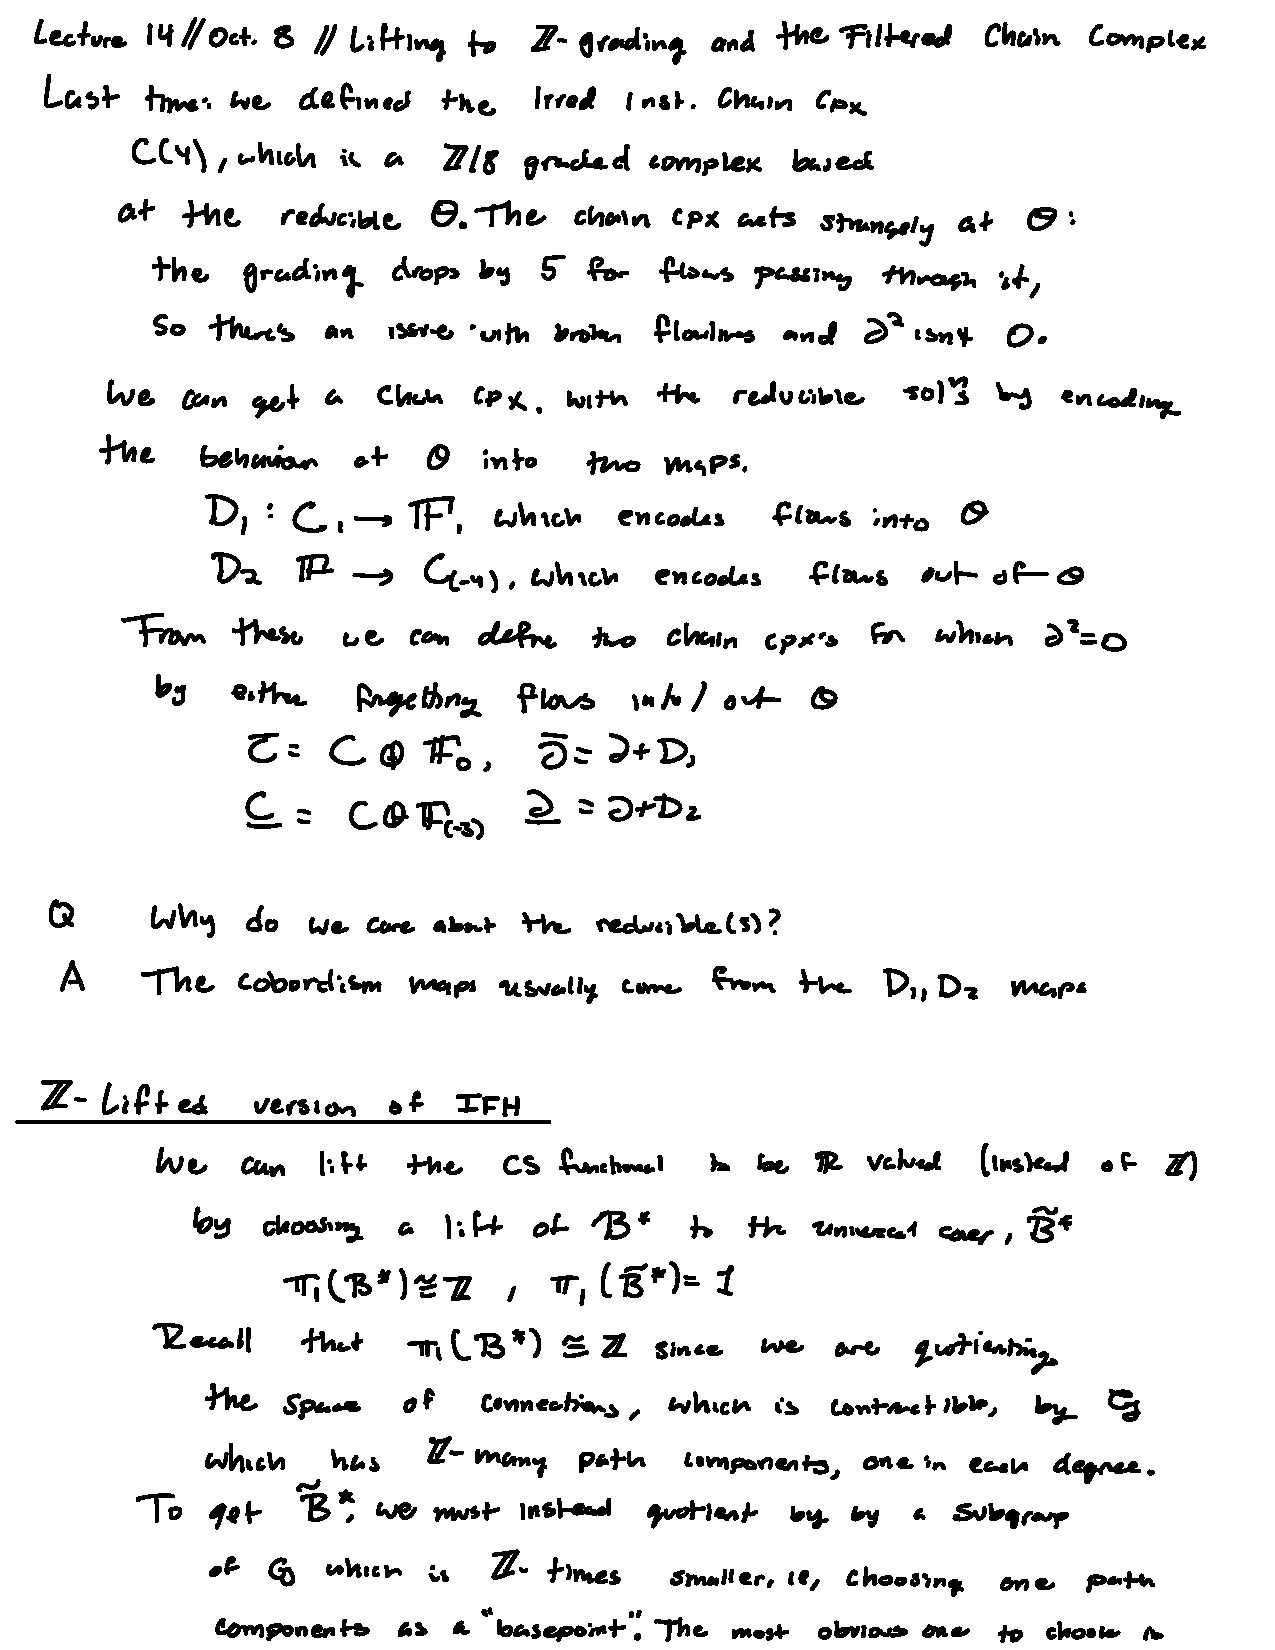
\includepdf[pages=-]{lecture14.pdf}

\end{document}
